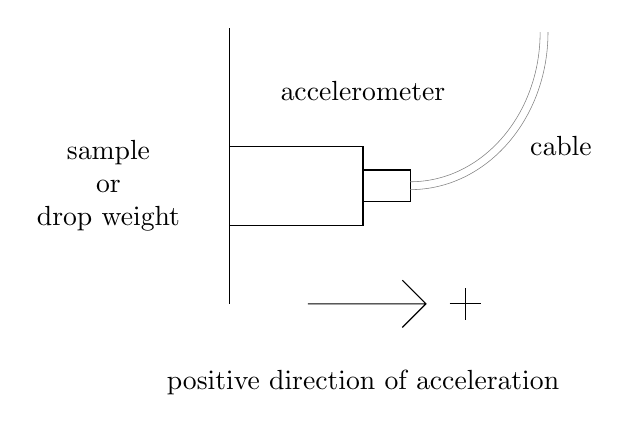
\begin{tikzpicture}

%wall
\draw (0,0.5) -- (0,1.5) 
(0,2.5) -- (0,4)

%accelerometer
(0,1.5) rectangle (1.7,2.5)
(1.7,1.8) rectangle (2.3,2.2);

%cable
\draw [help lines]
(2.3,1.95) arc [x radius = 1.75cm, y radius = 2cm, start angle= -90, end angle= 0]
(2.3,2.05) arc [x radius = 1.65cm, y radius = 1.9cm, start angle= -90, end angle= 0];

%text
\node at (1.7,3.2) {accelerometer};
\node at (3.7,2.5) [right] {cable};
\node at (-0.5,2) [left, align = center] {sample \\ or \\ drop weight};

%direction of positive acceleration
    %arrow
\draw
(1,0.5) -- (2.5,0.5)
(2.2,0.8) -- (2.5,0.5) -- (2.2,0.2);
    %plus
\draw (3,0.7) -- (3,0.3)
(2.8,0.5) -- (3.2,0.5);
    %text
\node at (1.7,-0.5) {positive direction of acceleration};

\end{tikzpicture}